\documentclass[11pt,xcolor=svgnames]{beamer}
\usepackage{dsfont,natbib,setspace,changepage,multirow}
\mode<presentation>

% replaces beamer foot with simple page number
\setbeamertemplate{navigation symbols}{}
%\setbeamerfont{frametitle}{series=\bfseries}
\setbeamercolor{frametitle}{fg=Black}

\setbeamertemplate{footline}{
   \raisebox{5pt}{\makebox[\paperwidth]{\hfill\makebox[20pt]{\color{gray}\scriptsize\insertframenumber}}}}

\usepackage{algorithm}
\usepackage{algorithmic}

% colors
\newcommand{\theme}{\color{Maroon}}
\newcommand{\bk}{\color{black}}
\newcommand{\rd}{\color{DarkRed}}
\newcommand{\fg}{\color{ForestGreen}}
\newcommand{\bl}{\color{blue}}
\newcommand{\gr}{\color{black!50}}
\newcommand{\sg}{\color{DarkSlateGray}}
\newcommand{\nv}{\color{Navy}}
\setbeamercolor{itemize item}{fg=gray}

% common math markups
\newcommand{\bs}[1]{\boldsymbol{#1}}
\newcommand{\mc}[1]{\mathcal{#1}}
\newcommand{\mr}[1]{\mathrm{#1}}
\newcommand{\bm}[1]{\mathbf{#1}}
\newcommand{\ds}[1]{\mathds{#1}}
\newcommand{\indep}{\perp\!\!\!\perp}
\def\plus{\texttt{+}}
\def\minus{\texttt{-}}

% spacing and style shorthand
\setstretch{1.1}

\begin{document}

\setcounter{page}{0}
{ \usebackgroundtemplate{
\includegraphics[height=\paperheight]{phoenix}}
\begin{frame}[plain]
\begin{center}

{\bf \LARGE \theme }

{\bf \Large  Big Data and Bayesian Nonparametrics}

\vskip 2cm
Matt Taddy,  Chicago Booth


\vskip .25cm
{\texttt{faculty.chicagobooth.edu/matt.taddy/research}}

\end{center}
\end{frame} }


\begin{frame}

{\bf Big Data}

\vskip .25cm

\vskip .25cm
{\nv The sample sizes are enormous.}
\begin{itemize}
\item We'll see 21 and 200 million today.  
\item Data can't fit in memory, or even storage, on a single machine.
%\item Our familiar MCMC algorithms take too long.
\end{itemize}


\vskip .25cm
{\nv The data are super weird.  }
\begin{itemize}
\item Internet transaction data distributions have a big spike at zero and spikes at other discrete values (e.g., 1 or \$99).
\item Big tails (e.g., \$12 mil/month eBay user spend) that matter.
\item The potential feature space is unmanageably large.
\item We cannot  write down or measure believable models.
\end{itemize}

\vskip .5cm\theme
Both `Big' and `Strange' beg for nonparametrics.

\end{frame}

\begin{frame}

{\bf what are nonparametrics?}

\vskip .5cm
There are many flavors.  One option is {\it distribution free NP:}


\vskip .15cm
1: Find some  statistic that is useful regardless of DGP.
\\{\nv (~DGP = Data Generating Process~)}


\vskip .15cm
2: Quantify {\theme uncertainty} about this stat under minimal assumptions.

\vskip .5cm
Practitioners apply the simple stat and feel happy that it will work.
 
\end{frame}


\begin{frame}

Our sample of data points $\bm{z}_i = [\bm{x}_i,y_i]$ is as good a guess as any at what the population DGP looks like. 
We can explore {\theme uncertainty} about this population by {\theme randomly re-weighting our sample}.

\begin{center}
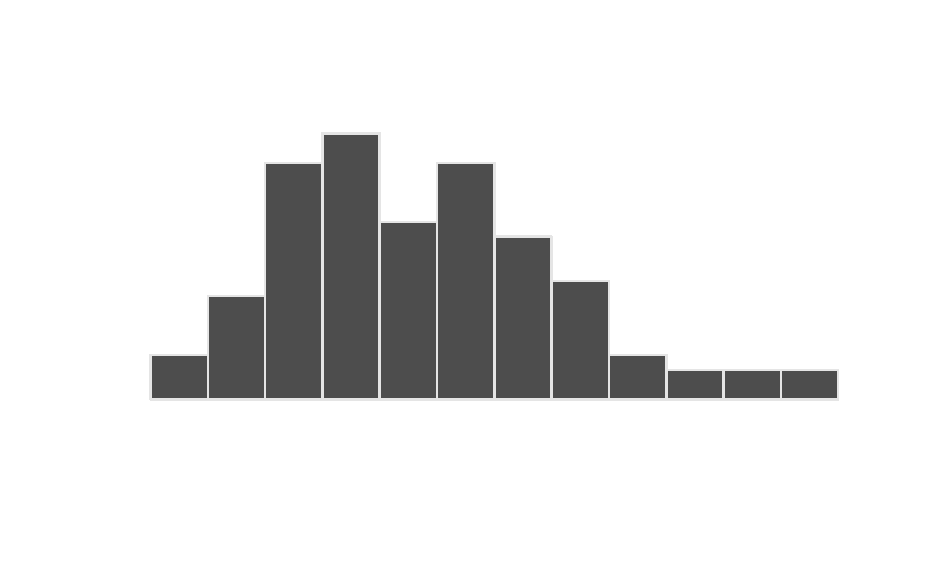
\includegraphics[width=2in]{graphs/bs_bighist}

{\gr data sample}

$\swarrow~~~\downarrow~~~\searrow$

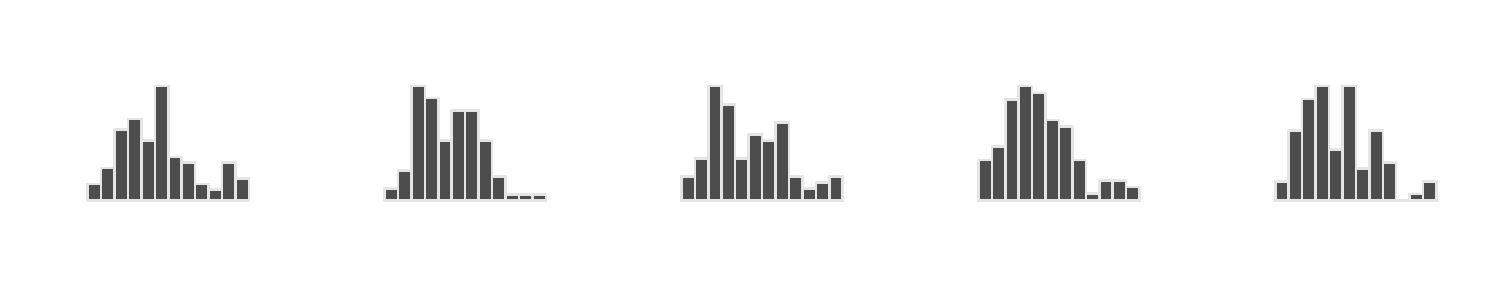
\includegraphics[width=4.25in]{graphs/bs_boothist}

\gr randomly re-weighted samples
\end{center}
\hfill
{This is just the Bayesian bootstrap. \gr (Rubin 1981)}

\end{frame}


\begin{frame}

{\bf {\gr Example:} Decision Trees}

\vskip .5cm
Trees are great: nonlinearity, deep interactions, heteroskedasticity.

\begin{center}
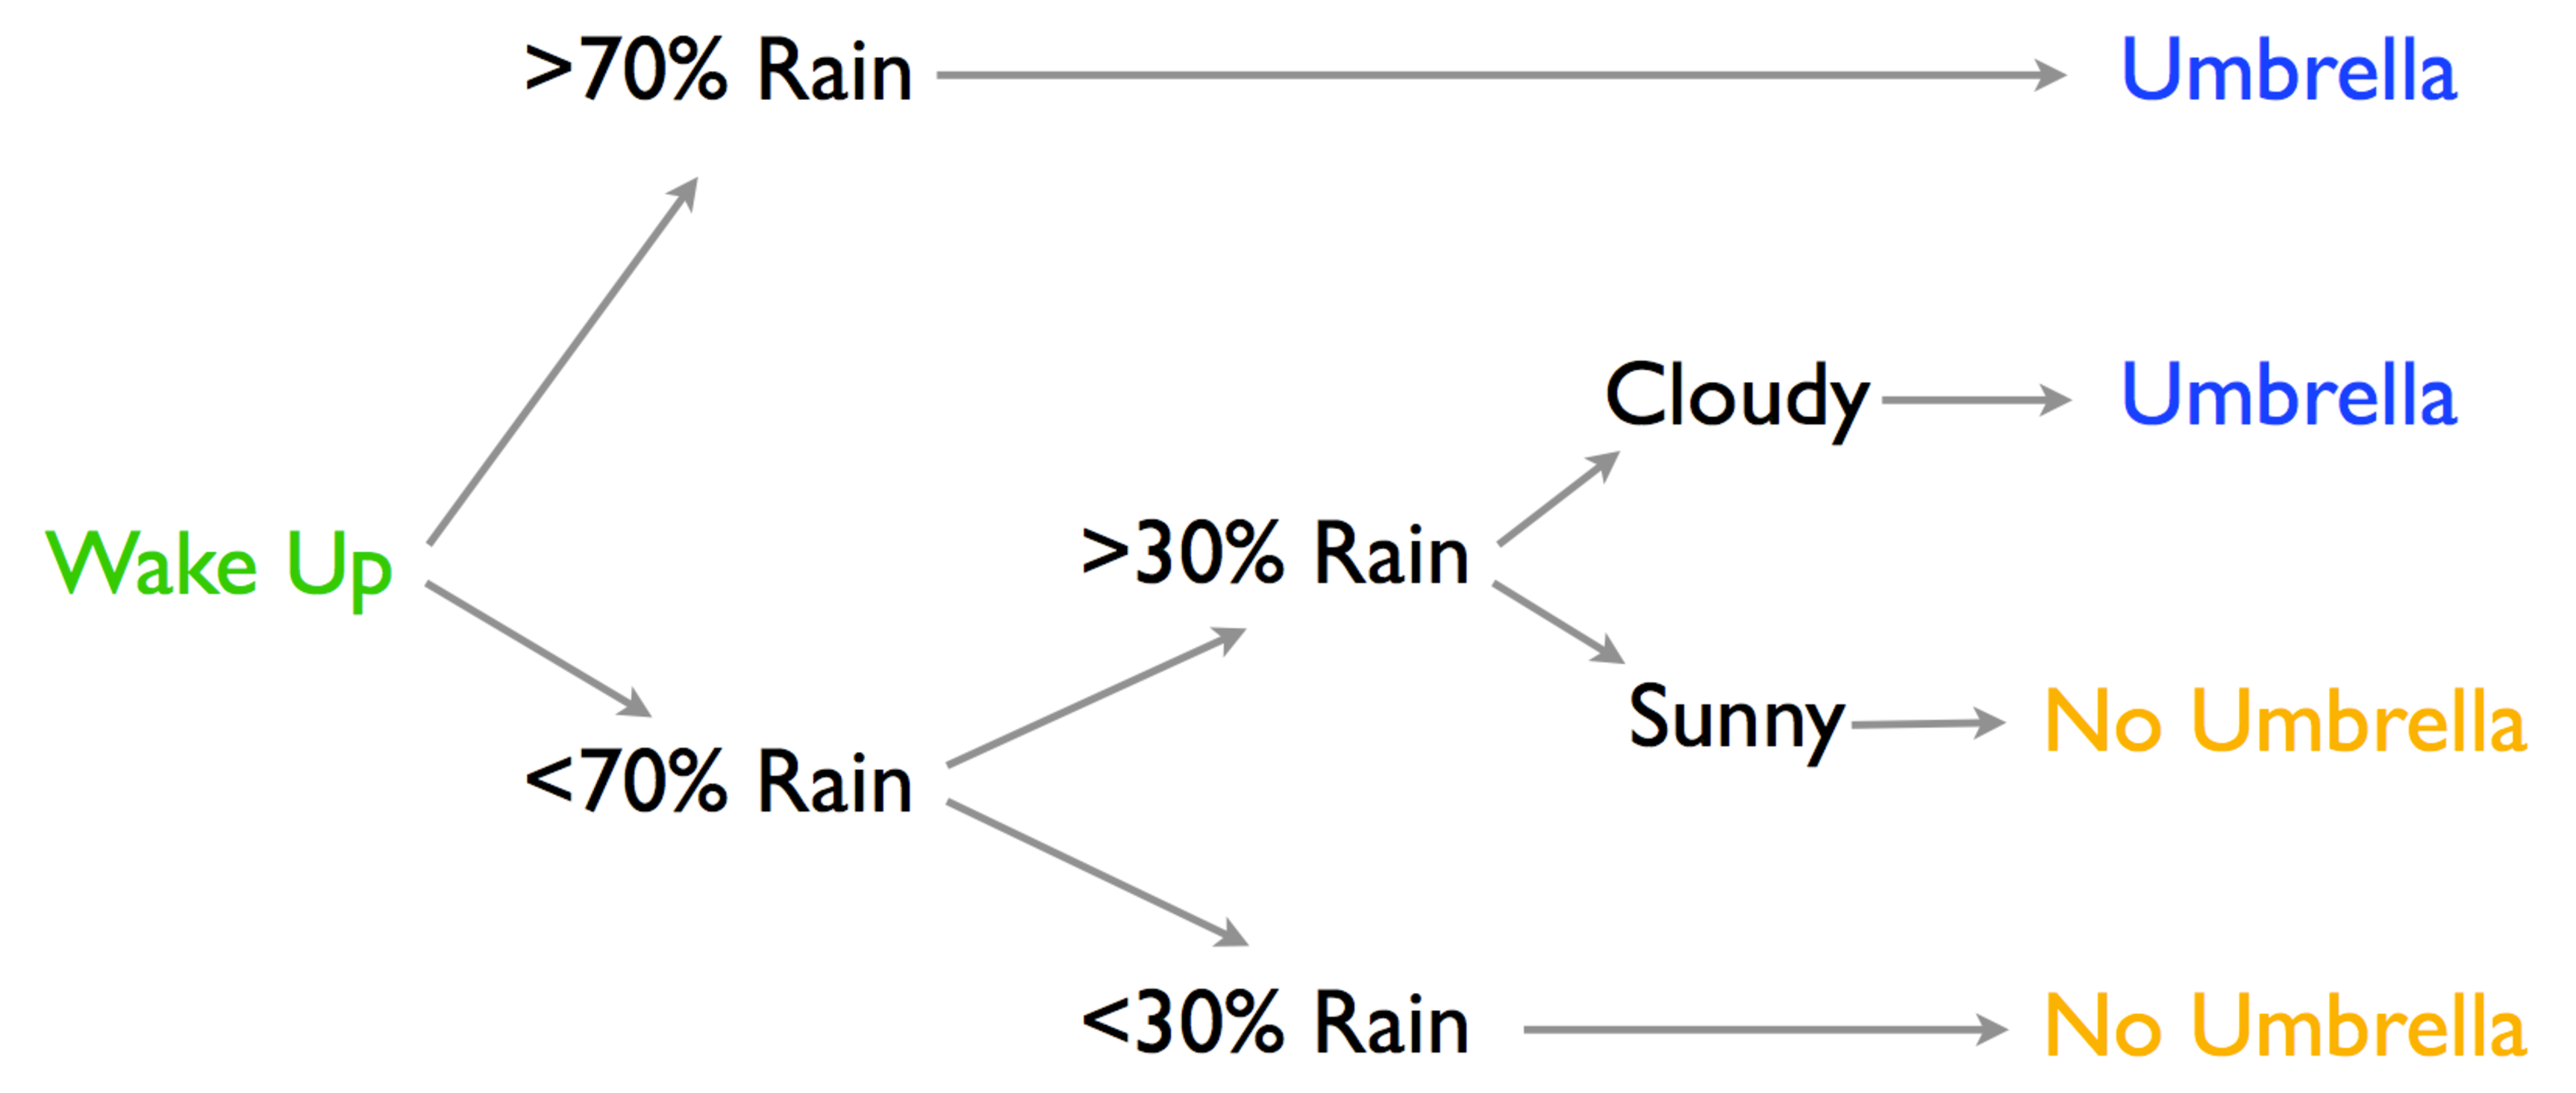
\includegraphics[width=4in]{graphs/umbrella}
\end{center}

The `optimal' decision tree is a statistic we care about {\gr (s.w.c.a)}.


\end{frame}


\begin{frame}


{\bf {\theme CART:} greedy growing with optimal splits}

\vskip .5cm
For any dataset, find the {\nv input} variable and dimension so that 
you can use $\leq$ or $>$ on this $x$ to minimize something like
\[
n_{\text{left}}\text{var}(\bm{z}_k: x_{kj}\leq x)+ n_{\text{right}}\text{var}(\bm{z}_k: x_{kj}> x)
\]

You  repeat this on  each of the (left and right) child {\nv nodes} \\until you get to {\nv leaves} that only contain a small set of data.

\vskip .5cm
{\theme Quantifying uncertainty:} do this, but for random reweightings of the data (i.e., so that those variances are now weighted sums).
\end{frame}



\begin{frame}

{\bf Forests}

\vskip .25cm
Each re-weighting yields a different tree.  We are left with a {\theme forest}.

\vskip .25cm
{\nv Fact:} the {\theme average} prediction from this forest is better than the prediction from any single tree.

\vskip .25cm
~~~~~~~~~~~~~~~~~~~~~{\it one tree~~~~~~~~~~~~~~~~~~~~~~~~~~~~~~~~~~posterior mean}\\

\includegraphics[height=1.75in]{graphs/MCtreedraw}   
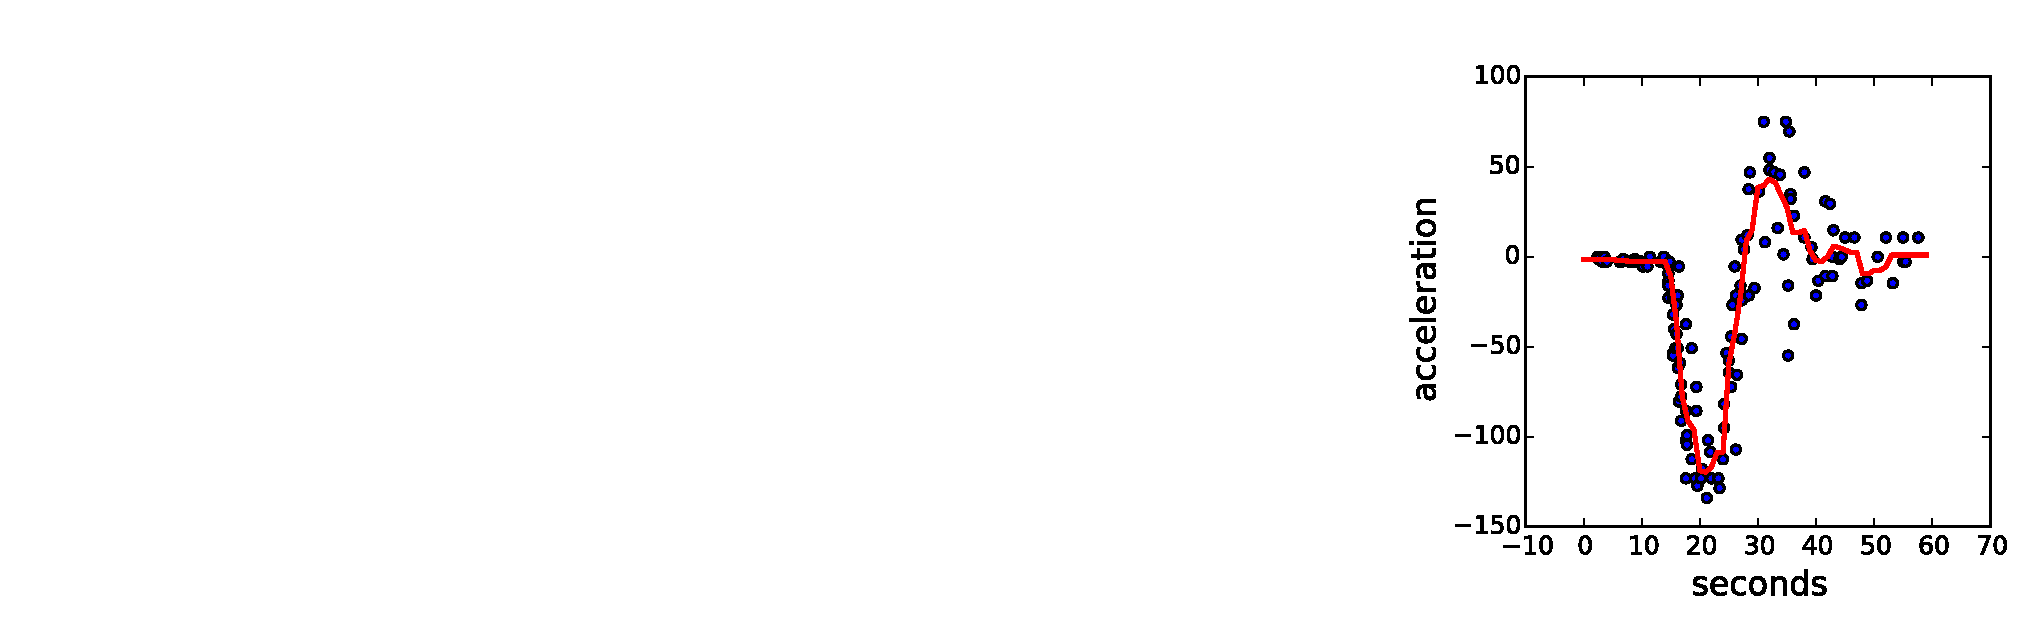
\includegraphics[height=1.75in]{graphs/MCbforest}   

\vskip .25cm{
Random Forest $\approx$ Bayesian forest $\approx$ posterior over CART fits.}
\end{frame}

\begin{frame}

{\bf Trunk stability}

\vskip .25cm
Based on this model for forests as randomly weighted CART, \\ we can derive a theory on the variance of trees.

\vskip .25cm
This yields that, for data at a given node, 
\begin{equation*}\theme
\mathrm{p}\left(\text{optimal split matches sample CART}\right) \gtrsim 1 - \frac{p}{\sqrt{n}} e^{-n},
\end{equation*}
with $p$ split locations and $n$ observations.  

\vskip .25cm
$\Rightarrow$ If we look at our {\it forest}, we  expect that the {\theme trunks} of the trees (the first few splits) will look the same across trees.

\end{frame}

\begin{frame}

{\bf California Housing Data}


\vskip .5cm

20k observations on median home prices in zip codes.

\vskip .5cm

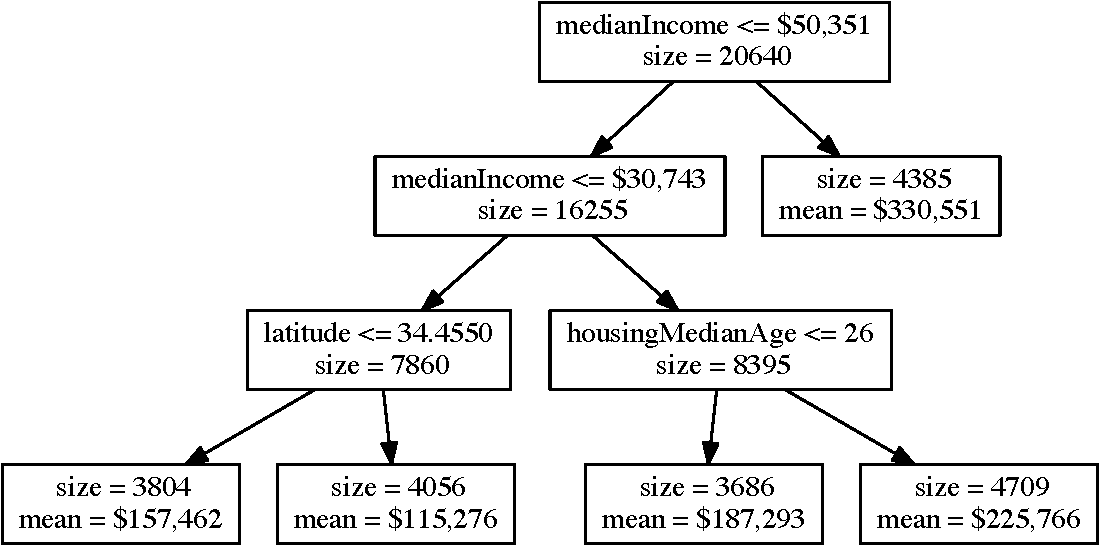
\includegraphics[width=\textwidth]{graphs/ca_trunk}

\vskip .5cm
\hfill Above is the trunk you get setting min-leaf-size of 3500.

\end{frame}

\begin{frame}

\begin{columns}

\begin{column}{2.15in}
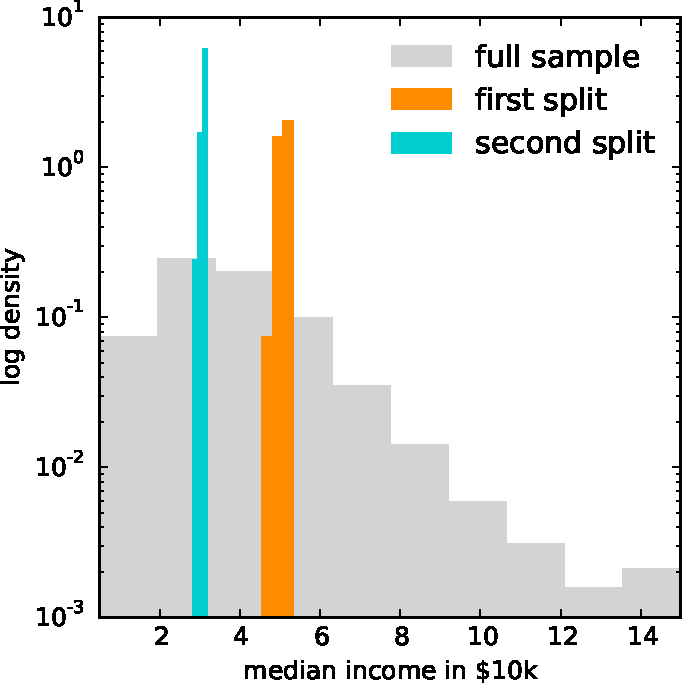
\includegraphics[width=2.5in]{graphs/ca_splits}
\end{column}

\begin{column}{2in}
\begin{itemize}
\item sample tree occurs 62\% \\of the time.  
\vskip .5cm
\item 90\% of  trees split on income twice, \\and then latitude. 

\vskip .5cm
\item 100\% of trees have 1st 2 splits on median income.  
\end{itemize}
\end{column}

\end{columns}


\vskip 1cm
~~~~Empirically and theoretically: trees are stable, at the trunk.
\vskip -1cm

\end{frame}

\begin{frame}

{\bf Random Forest {\theme bottlenecks}}

\vskip .5cm
RFs (or BFs) are awesome, but when the data are too big to fit in memory or on a single machine they get extremely expensive.\\ {\gr \small (e.g., Google PLANET, Panda 2009)}.

\vskip .5cm
A common solution is a `sub-sampling forest': instead of drawing with-replacement, or re-weighting, draw $m \ll n$ sub-samples.

\vskip .5cm
This defeats the whole purpose of trees: these are rules that are designed to grow in complexity with the amount of data available. {\gr(that's why we bother storing so much data!)}

\vskip .5cm If you starve the individual trees of data you lose.

\end{frame}

\begin{frame}
\begin{adjustwidth}{-.5in}{}
\vskip -.6in
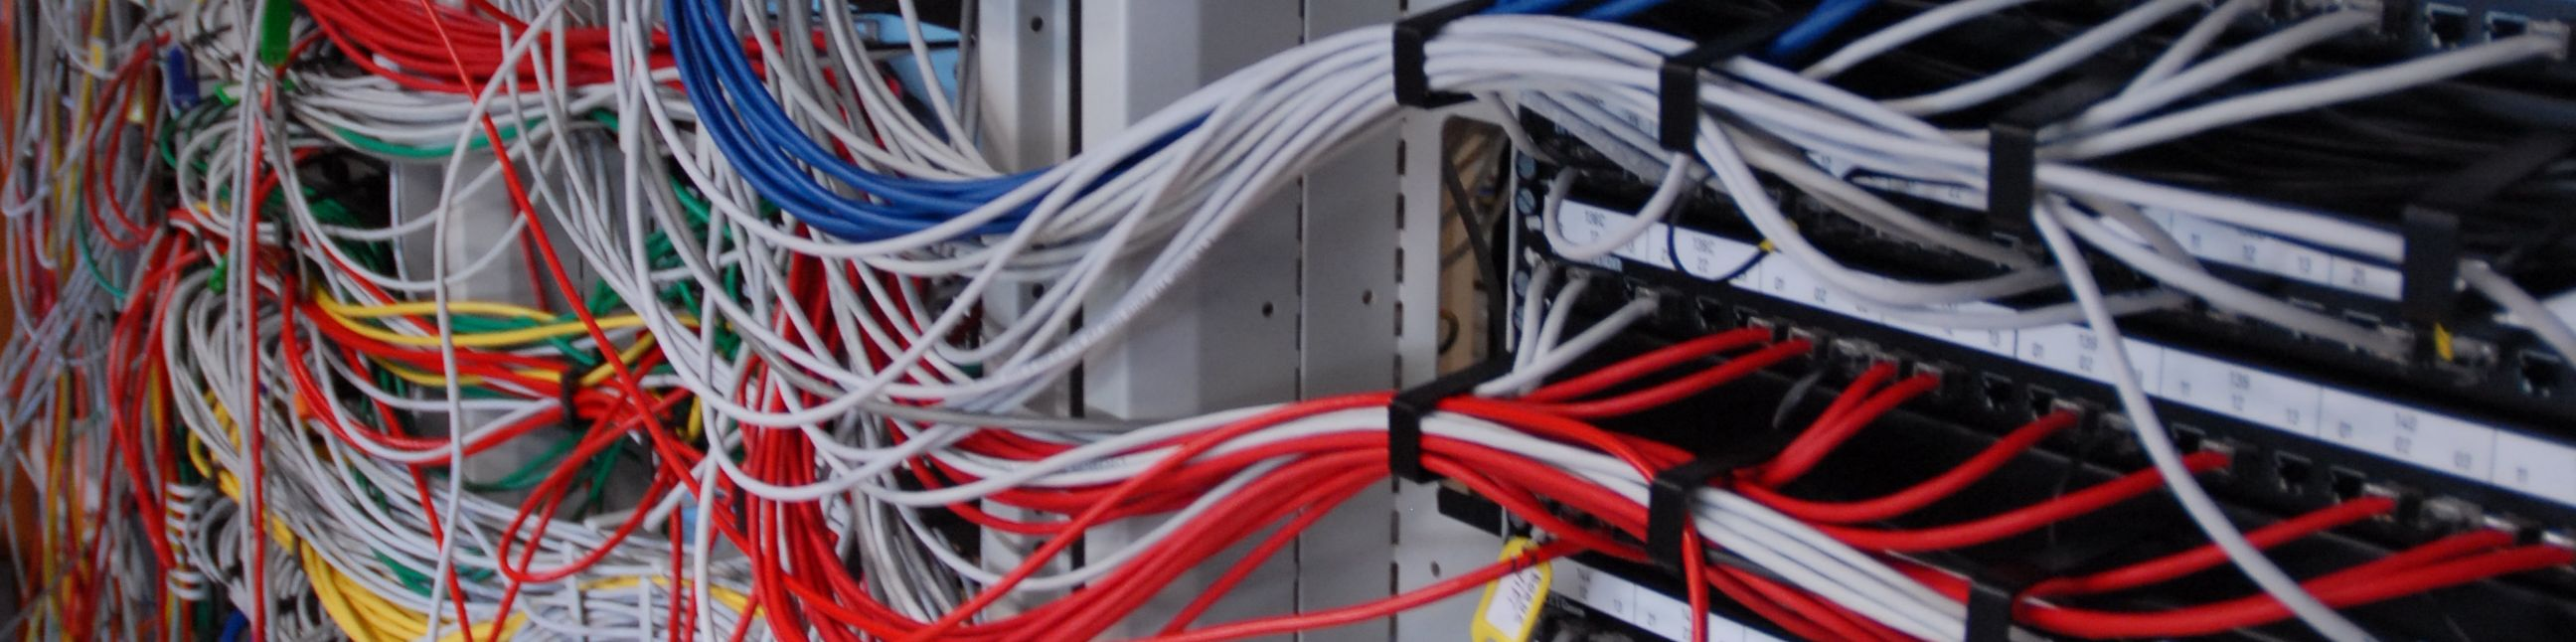
\includegraphics[width=6in]{graphs/broadband}
\end{adjustwidth}

\vskip .6cm

{ \bf Data Distribution and Big Data}

\vskip .5cm
{\nv Distributed}: independent computations on many datasets.\\

\vskip .1cm
For truly {\nv Big Data} we need distributed algorithms.

\vskip .5cm
The trick is to find strategies for distribution so that local-machine calculations are as relevant as possible to the global inference question:
only data that needs to be together is together.

\end{frame}



\begin{frame}

{\bf Empirical Bayesian Forests ({\theme EBF})}

\vskip .5cm
RFs are expensive.  Sub-sampling hurts bad.

\vskip .25cm
{Instead:}
\begin{itemize}
\item fit a single tree to a shallow {\nv trunk}.  
\item Map data to each {\nv branch}.  
\item Fit a full  forest on the smaller branch datasets.
\end{itemize}

\vskip .25cm
Since the trunks are all similar for each tree in a full forest,
our EBF looks nearly the same at a fraction of computational cost.

\vskip .5cm
It's an updated version of classical {\theme Empirical Bayes}: \\ ~~~use plug-in estimates at high levels in a hierarchical model, \\~~~focus effort at full Bayesian learning for the the hard bits.


\end{frame}

\begin{frame}

{\bf OOS predictive performance on California Housing}




\begin{center}
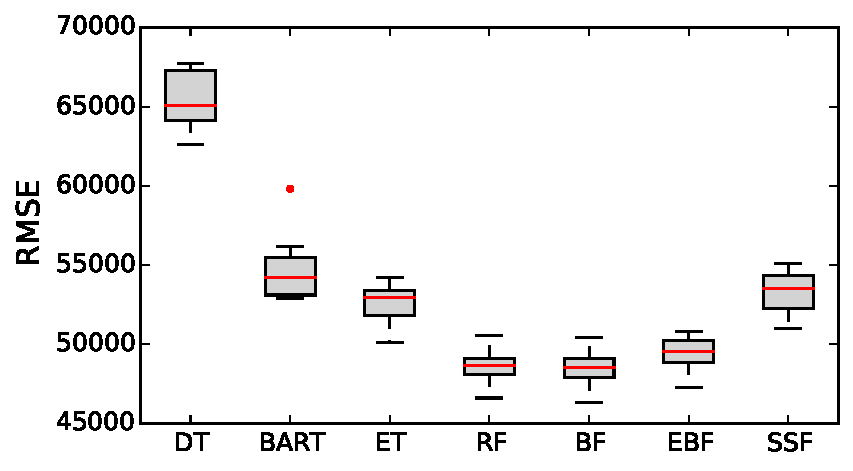
\includegraphics[width=.85\textwidth]{graphs/ca_rmse}
\end{center}

Here EBF and BF give nearly the same results.  {\it SSF does not.}

\vskip .25cm
EBFs crunch more data faster without hurting performance.


\end{frame}


\begin{frame}

{\bf Catching {\theme Bad Buyer Experiences } at eBay}

\vskip .5cm
BBE: `not as described', delays, etc.

\vskip .1cm
$\mathrm{p}(\text{BBE})$
is a key input to search rankings, and elsewhere.

\vskip .5cm
Big Data axiom:  best way to improve prediction is more data.  

\vskip .1cm 
{\gr (a.k.a. `data beats model' )}


\vskip .5cm
On 200 million transactions,  EBF with 32 branches yields a\\ 1.5\% drop in misclassification over the SSF alternatives.  

\vskip .5cm
EBFs via Spark $\Rightarrow$ more data in less time.
\vskip .1cm 
Putting it into production requires some careful engineering, \\but this really is a very simple algorithm.  {\theme Big gain, little pain.} 

\end{frame}



\begin{frame}

{\bf Efficient Big Data analysis}

\vskip .25cm
To cut computation without hurting performance, we need to think about what portions of the `model' are {\theme hard} or {\nv easy} to learn.

\vskip .25cm
Once we figure this out,  we can use a little bit of the data to\\ learn the easy stuff and direct our full data at the hard stuff.

\vskip .25cm
This is {\it the} future for Big Data.

\hfill \huge \theme \bf thanks!

\end{frame}



\end{document}






























